\section*{Double Gauss Simulations}

Collection of simulations performed with the double gauss, currently without further comment. Number of fits retained is 868, 833, and 866 for the no delay, normal distribution, and weibull, respectively.

\subsection{No Delay}


\begin{figure}[H]
\centering
    \subfigure[]{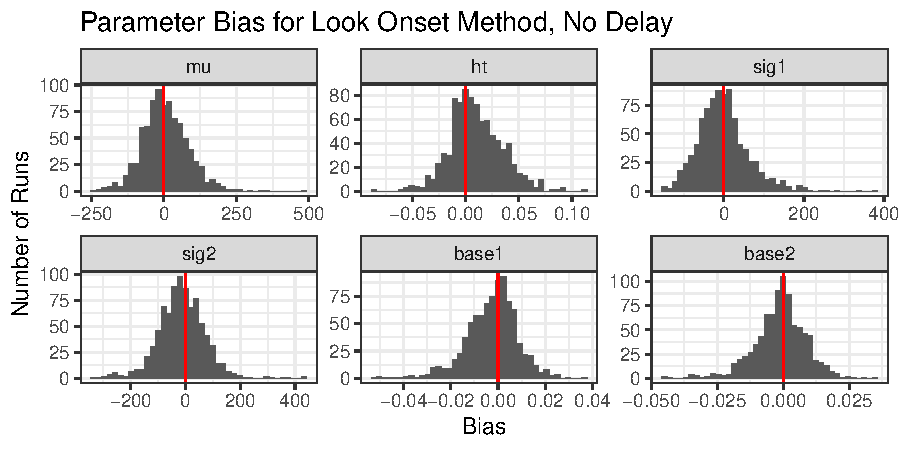
\includegraphics[width=0.9\textwidth]{dg_no_delay_par_bias_onset.pdf}} 
    \subfigure[]{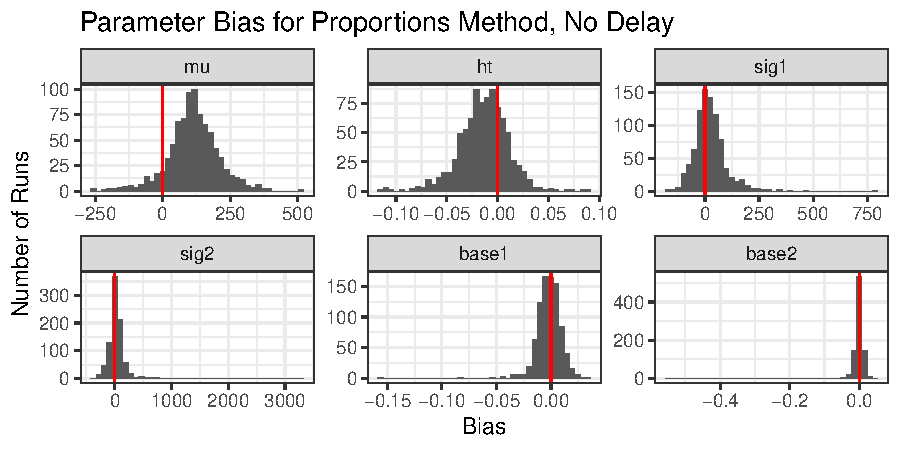
\includegraphics[width=0.9\textwidth]{dg_no_delay_par_bias_proportion.pdf}} 
\caption{Parameter bias for no oculmotor delay. }
\label{fig:dg_par_bias_no_delay}
\end{figure}

\begin{figure}[H]
\centering
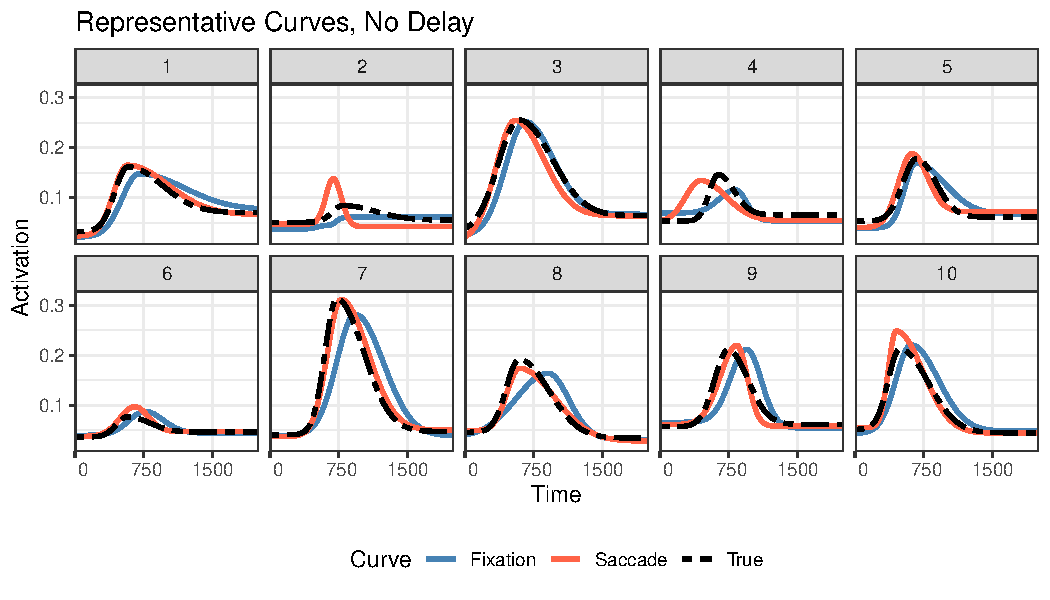
\includegraphics[width=0.9\textwidth]{dg_rep_curves_no_delay.pdf}
\caption{Representative curves for no oculmotor delay}
\label{fig:dg_rep_curves_no_delay}
\end{figure}


\subsection{Normal Delay}


\begin{figure}[H]
\centering
    \subfigure[]{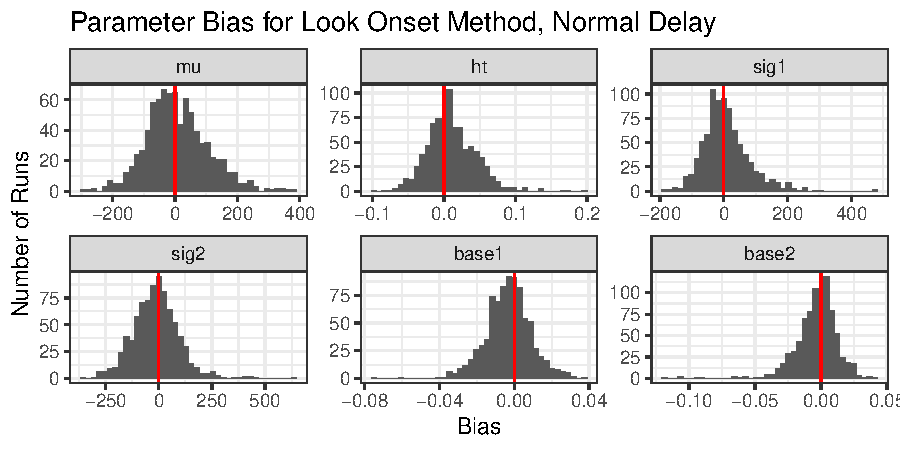
\includegraphics[width=0.9\textwidth]{dg_normal_delay_par_bias_onset.pdf}} 
    \subfigure[]{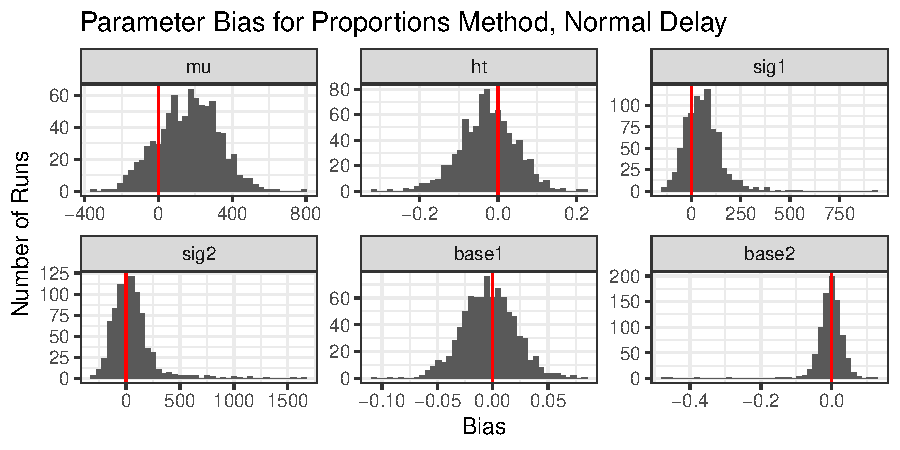
\includegraphics[width=0.9\textwidth]{dg_normal_delay_par_bias_proportion.pdf}} 
\caption{Parameter bias for normal OM delay}
\label{fig:dg_par_bias_normal_delay}
\end{figure}

\begin{figure}[H]
\centering
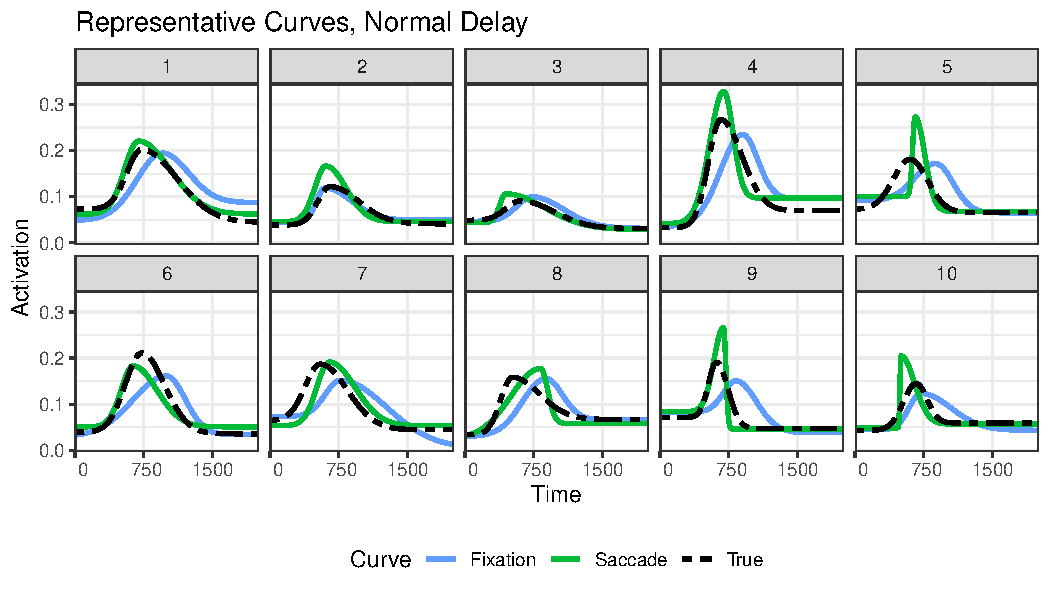
\includegraphics[width=0.9\textwidth]{dg_rep_curves_normal_delay.pdf}
\caption{Representative curves for normal oculomotor delay}
\label{fig:dg_rep_curves_normal_delay}
\end{figure}

\subsection{Weibull Delay}

\begin{figure}[H]
\centering

    \subfigure[]{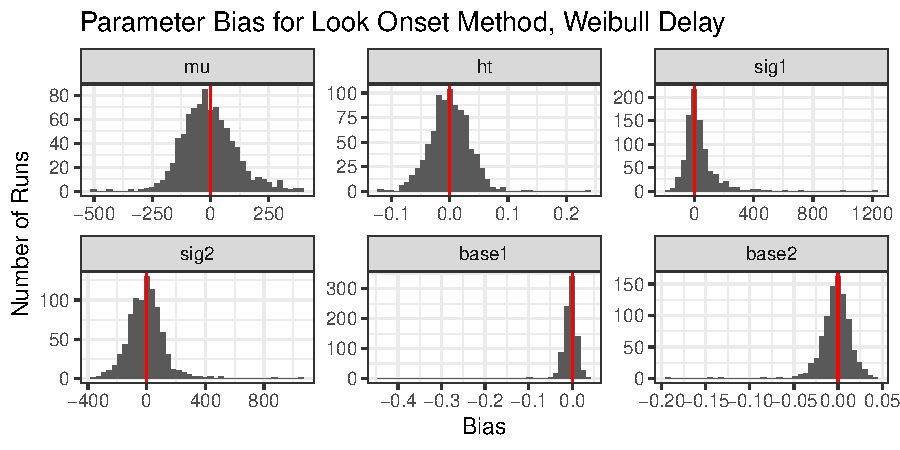
\includegraphics[width=0.9\textwidth]{dg_weibull_delay_par_bias_onset.pdf}} 
    \subfigure[]{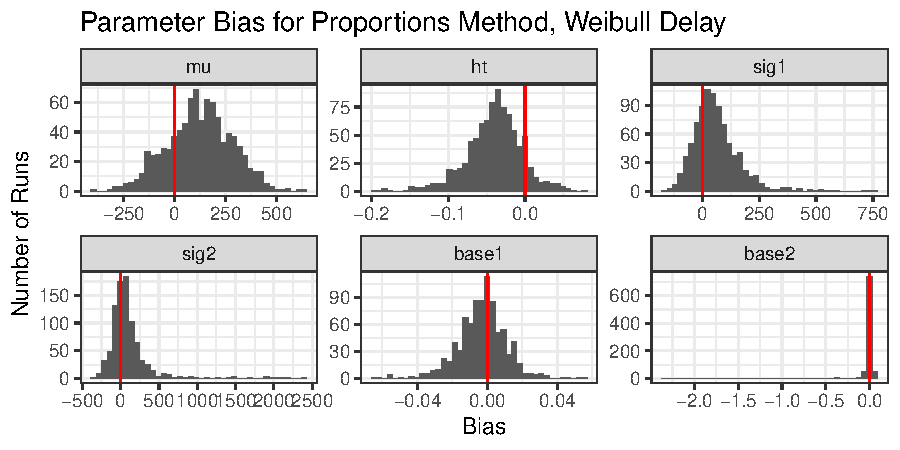
\includegraphics[width=0.9\textwidth]{dg_weibull_delay_par_bias_proportion.pdf}} 
\caption{Parameter bias for weibull OM delay}
\label{fig:dg_par_bias_weibull_delay}
\end{figure}

\begin{figure}[H]
\centering
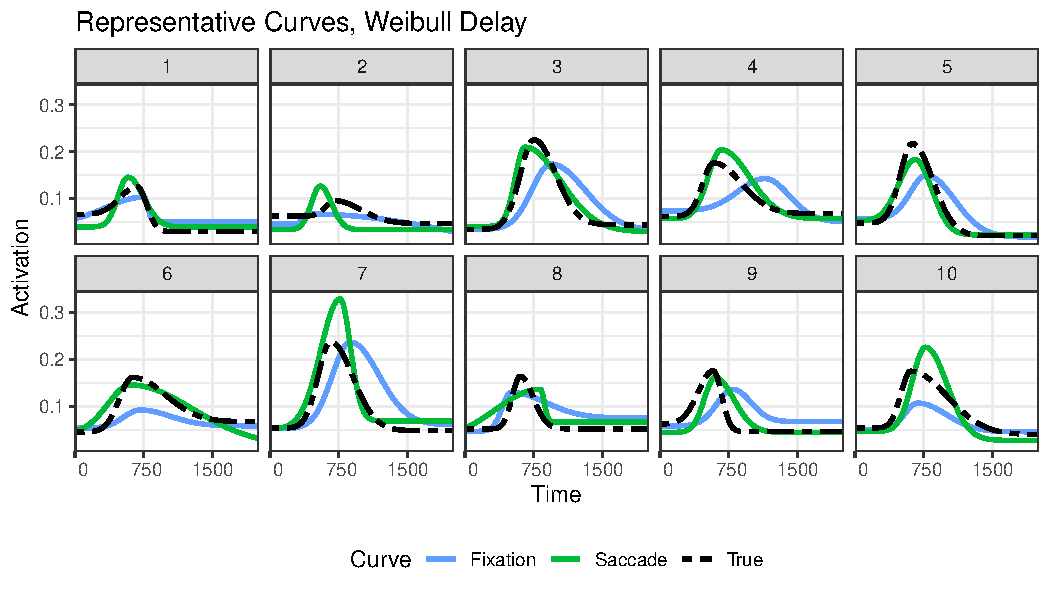
\includegraphics[width=0.9\textwidth]{dg_rep_curves_weibull_delay.pdf}
\caption{Representative curves for weibull oculmotor delay}
\label{fig:dg_rep_curves_weibull_delay}
\end{figure}
\subsection{Results}

\begin{table}[ht]
\centering
\begin{tabular}{llrrr}
  \hline
Curve & Delay & 1st Qu. & Median & 3rd Qu. \\ 
  \hline
Look Onset & No Delay & 0.22 & 0.36 & 0.63 \\ 
  Look Onset & Normal Delay & 0.38 & 0.70 & 1.15 \\ 
  Look Onset & Weibull Delay & 0.52 & 0.84 & 1.39 \\ 
  Proportion & No Delay & 0.75 & 1.29 & 2.08 \\ 
  Proportion & Normal Delay & 1.38 & 2.44 & 3.96 \\ 
  Proportion & Weibull Delay & 1.00 & 1.98 & 3.43 \\ 
   \hline
\end{tabular}
\caption{Figures not as striking as logistic, but keep in mind that the scale of this is significantly smaller, peaking at around 0.15 and being close to zero elsewhere. $R^2$ is another metric available}
\label{tab:dg_mise_sims}
\end{table}

\section*{$R^2$ instead of MISE for logistic/doublegauss}


\subsubsection{for logistic}

\begin{table}[H]
\centering
\begin{tabular}{llrrr}
  \hline
Curve & Delay & 1st Qu. & Median & 3rd Qu. \\ 
  \hline
Look Onset & No Delay & 1.00 & 1.00 & 1.00 \\ 
  Look Onset & Normal Delay & 0.99 & 1.00 & 1.00 \\ 
  Look Onset & Weibull Delay & 0.98 & 0.99 & 0.99 \\ 
  Proportion & No Delay & 0.92 & 0.94 & 0.95 \\ 
  Proportion & Normal Delay & 0.80 & 0.83 & 0.86 \\ 
  Proportion & Weibull Delay & 0.80 & 0.86 & 0.91 \\ 
   \hline
\end{tabular}
\caption{$R^2$ for logistic, not as clear a hierarchy}
\label{tab:r2_logistic_sims}
\end{table}

\subsubsection{for doublegauss}

\begin{table}[H]
\centering
\begin{tabular}{llrrr}
  \hline
Curve & Delay & 1st Qu. & Median & 3rd Qu. \\ 
  \hline
Look Onset & No Delay & 0.80 & 0.91 & 0.95 \\ 
  Look Onset & Normal Delay & 0.63 & 0.82 & 0.91 \\ 
  Look Onset & Weibull Delay & 0.57 & 0.77 & 0.87 \\ 
  Proportion & No Delay & 0.48 & 0.65 & 0.75 \\ 
  Proportion & Normal Delay & 0.10 & 0.33 & 0.52 \\ 
  Proportion & Weibull Delay & 0.20 & 0.46 & 0.64 \\ 
   \hline
\end{tabular}
\caption{$R^2$ for double gauss}
\label{tab:r2_dg_sims}
\end{table}
